\section{Methods}
\label{methods}

When applied to spectral fitting, Bayesian algorithms aim to infer the posterior probability distributions $P(\theta \mid x)$ of galaxy properties, $\theta$, given observations, $x$. For a specific $\theta$ and $x$, one typically evaluates the posterior using Bayes' rule, $P(\theta \mid x) \propto P(\theta) \; P(x \mid \theta)$, where $P(\theta)$ denotes the prior distribution and $P(x \mid \theta)$ the likelihood, usually assumed to have a Gaussian functional form:


\begin{equation}
\log P(x \mid \theta)=-\frac{1}{2}(x-m(\theta))^T C^{-1}(x-m(\theta)),
\end{equation}




where $m(\theta)$ is the theoretical model, in our case a galaxy spectral model, and $C$ is the covariance matrix of the observations. \\

Simulation-based inference (SBI), also known as likelihood-free inference, offers an alternative that requires no assumptions about the form of the likelihood. In a nutshell, it consists of creating synthetic data, often called the forward model,  and then fitting them like real observations, the backward model, comparing against a known ‘truth’. Therefore, SBI uses a generative model, i.e. a simulation $F$, to generate mock data $x^{\prime}$ given parameters $\theta^{\prime}: F\left(\theta^{\prime}\right)=x^{\prime}$. It uses a large number of simulated pairs $\left(\theta^{\prime}, x^{\prime}\right)$ to directly estimate either the posterior $P(\theta \mid x)$, the likelihood $P(x \mid \theta)$, or the joint distribution of the parameters and data $P(\theta, x)$. This technique has already been applied successfully to several Bayesian parameter inference problems in astronomy \citep[e.g.][]{Cameron_2012, mishrasharma2022inferring, hahn23,zhang23}.\\

 The SBI approach can help us deal with the parameter space coverage, as most observations are unbalanced and affected by selection effects, and do not allow to obtain the kind of broad and uniform dataset usually required by inference algorithms. Moreover, SBI is especially useful when testing single-effect biases (e.g., parametrizations of SFHs or noise), enabling to layer complexity. In contrast, it is likely to generate problems of domain shifts when generalising results to real observations. Modelling considerations, like priors, wavelength coverage, or resolution, can have a significant impact on inferred galaxy properties \citep{Leja_2019,Hahn_2022} and must be carefully selected.\\ 


\subsection{Forward model}
\label{forward}

The first step is to generate a synthetic dataset to train and test our model, for which the spectrum, the SFH, and the metallicity are known. We work with MILES SPS models \citep{Vazdekis_2010}.  These fully empirical SSP models provide medium resolution \citep[$\text{FWHM}=2.51\AA$,][]{falcon11} predictions for a wide range of ages (from $0.03$ Gyr to $14.00$ Gyr) and metallicities ($\rm{[M/H]}$ moving from $-2.27$ to $0.40$). We select a Kroupa universal IMF and BaSTI isochrones, in the wavelength range $[3540.5,7409.6] \, \AA$, and use the so-called base models for $[\alpha/\rm{Fe}]$, following the abundance pattern of the solar neighbourhood.\\

We build physically-motivated non-parametric SFHs with Dense Basis \citep{Iyer_2017}, specifically the module GP-SFH. These SFHs allow complex behaviours like rejuvenation events, bursts or sudden quenching, and do not rely on a fixed functional form. The selected prior assumes that the fractional specific SFR (sSFR, i.e. the SFR normalised by the stellar mass), for three equally spaced time bins, follows a Dirichlet distribution \citep{Leja_2017} with a concentration parameter $\alpha=1$. Moreover, a uniform prior is included for the logarithm of the total stellar mass, $8.0 \leq \text{log} \left(M_{*}/M_{\odot}\right) \leq 12.0$, and for the logarithm of the sSFR at $z=0$, $-17.0 \leq \text{log} \left(\text{sSFR}/ \rm{yr}^{-1}\right) \leq -7.5$. We believe that these priors are general enough not to impose strong effects on the measurements, however, they will always play a role in the model predictions.\\


For simplicity we assume that there is no time evolution in metallicity, so each SFH is assigned with a single value of $\rm{[M/H]}$. We interpolate MILES spectra in time to obtain a SSP spectrum each $0.01347$ Gyr, with cosmic time in the range $[0.00,13.47]$ Gyr ($1{,}000$ time bins). In addition, as the metallicity bins of the spectral library are not equally spaced, which may cause problems when introducing the spectra to the network, we interpolate them in $\rm{[M/H]}$ too, obtaining $15$ equally spaced values of this parameter in the range $[-2.3,0.4]$. For each artificial SFH, given a value of $\rm{[M/H]}$, all the MILES interpolated spectra (corresponding to different ages and with that metallicity) are combined as:

\begin{equation}
\resizebox{.49 \textwidth}{!} 
{$
F_{\text{gal}} \left( \lambda,M_{\text{tot}},\rm{[M/H]},[\alpha / Fe]_{\text{Base}} \right) =\displaystyle \sum_{t_i} \frac{M(t_i)}{M_{\text{tot}}} \cdot F_{\text{SSP}} \left( \lambda,t_i,{\rm{[M/H]}},[\alpha/\rm{Fe}]_{\text{Base}}  \right)
$.}
\end{equation}

Finally, each spectrum is normalised by its median. In total, we obtain $10{,}000$ SFHs for each value of $\rm{[M/H]}$, so: $10{,}000$ SFHs x $15$ bins of metallicity $= 150{,}000$ spectra, for which SFHs and metallicities are known. Examples of the mock SFHs and their corresponding spectra are shown in Fig.~\ref{input}.\\

\begin{figure*}[h]
    \centering
    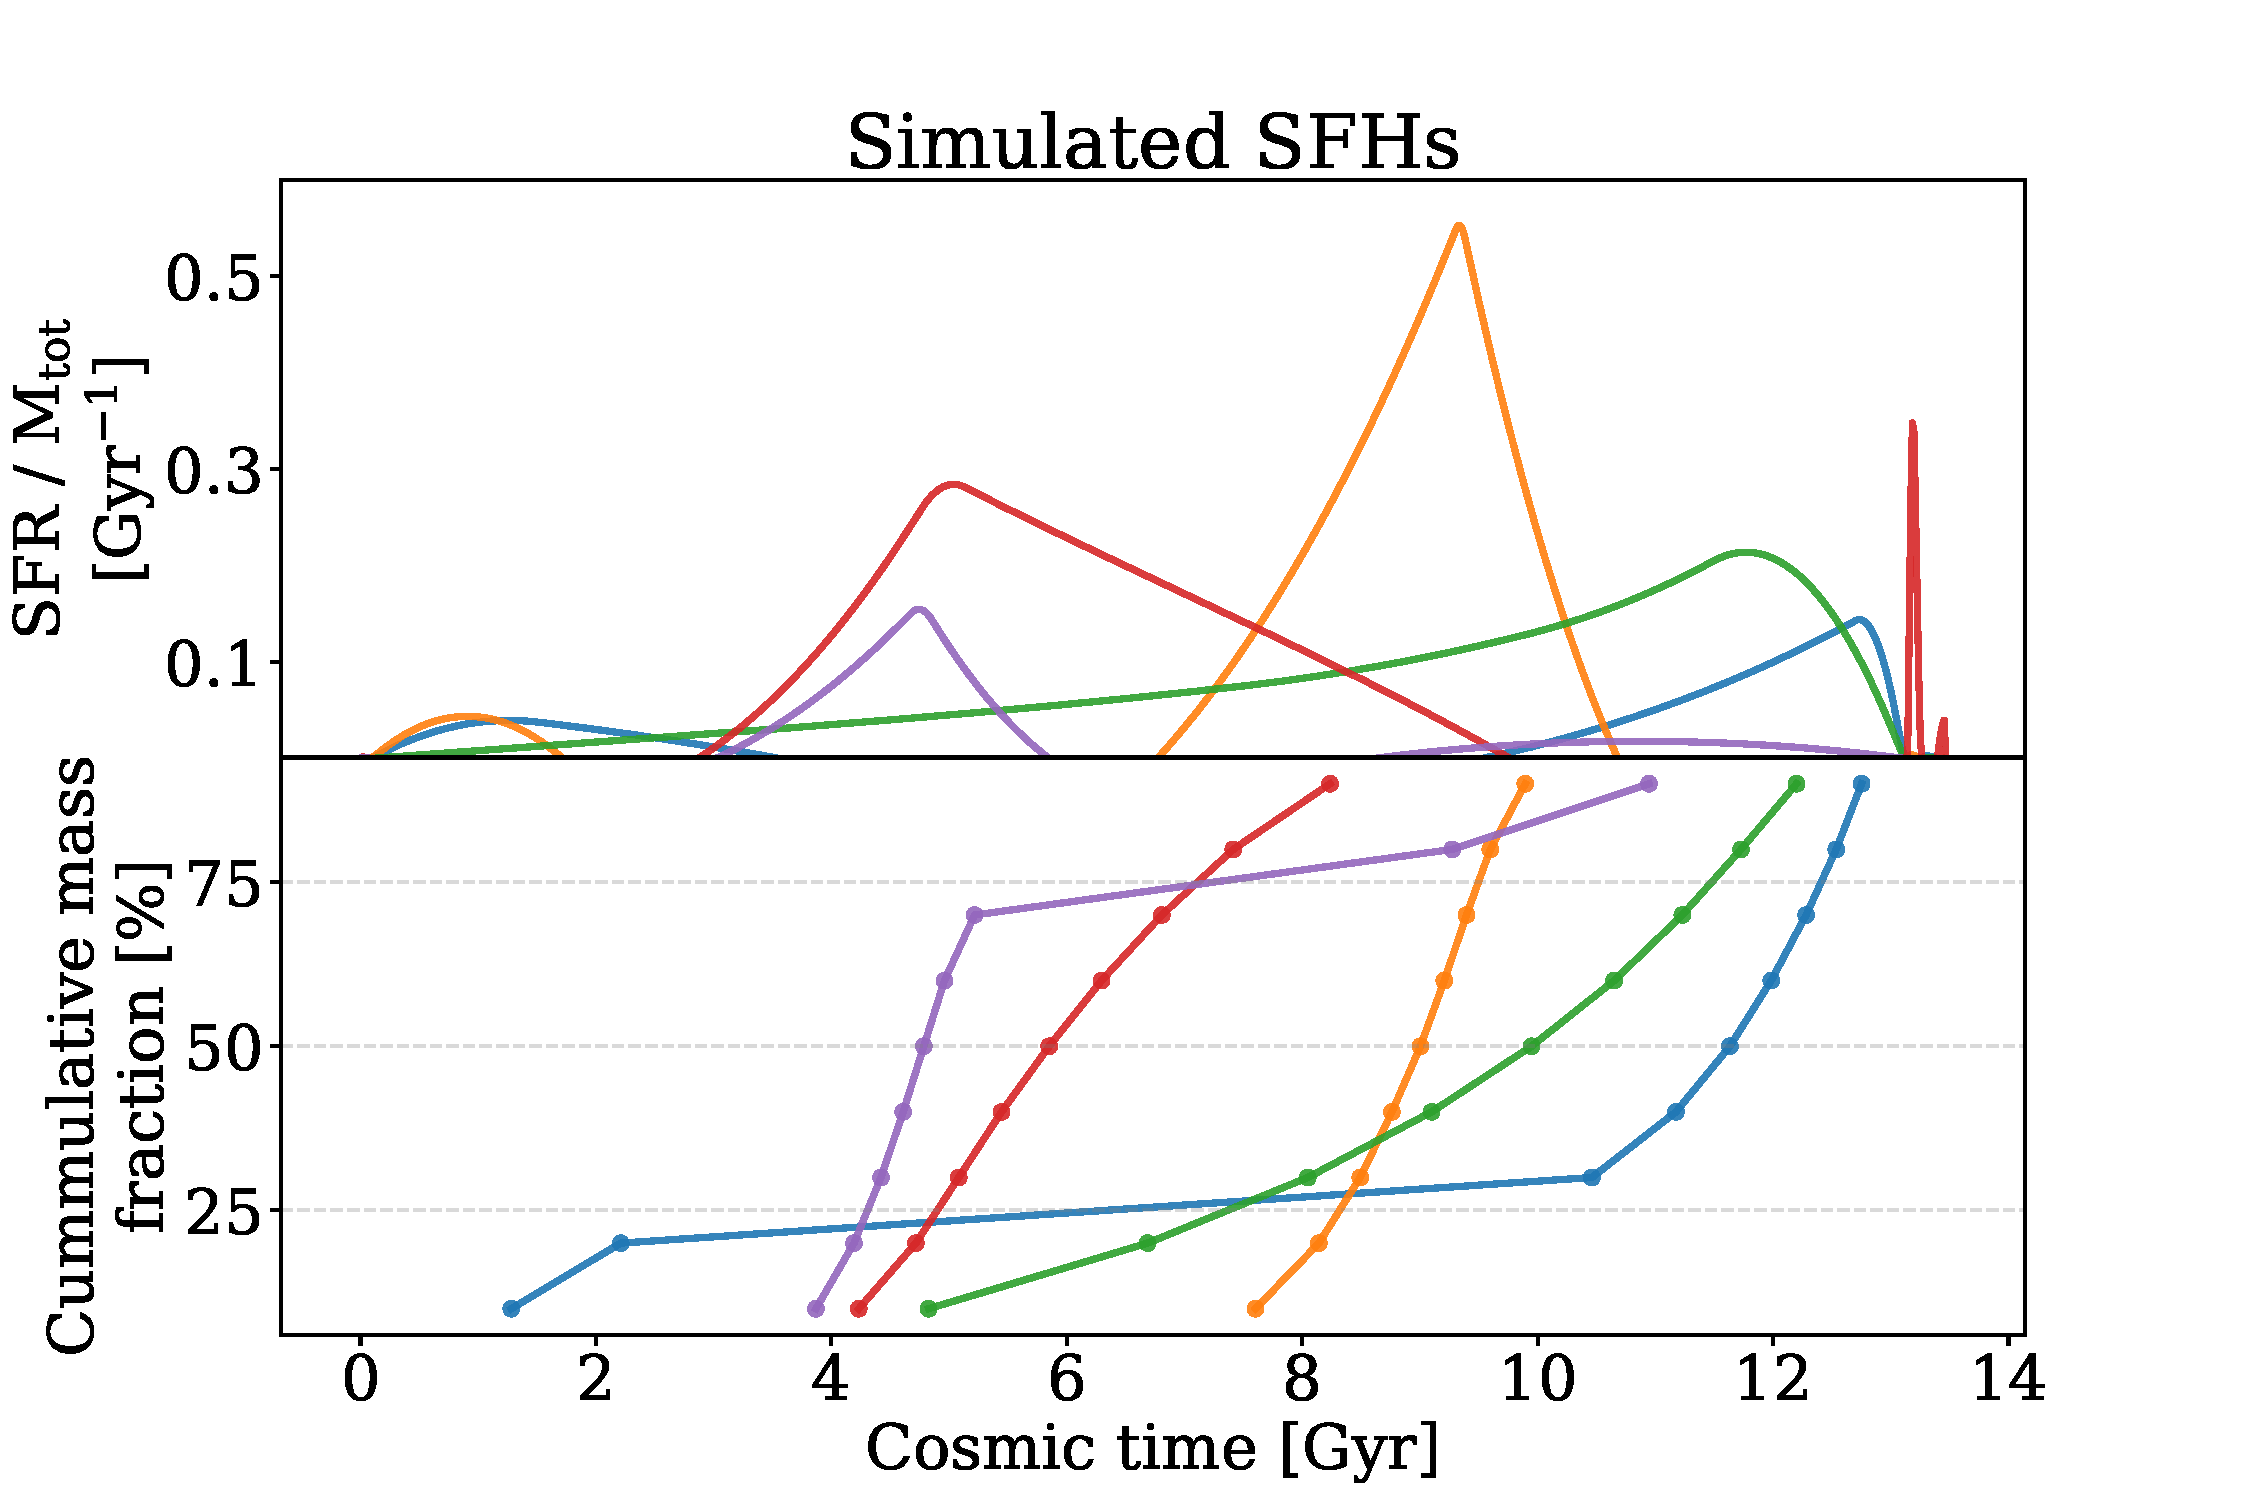
\includegraphics[width=0.49\textwidth]{images/input/sim_sfhs.pdf}
    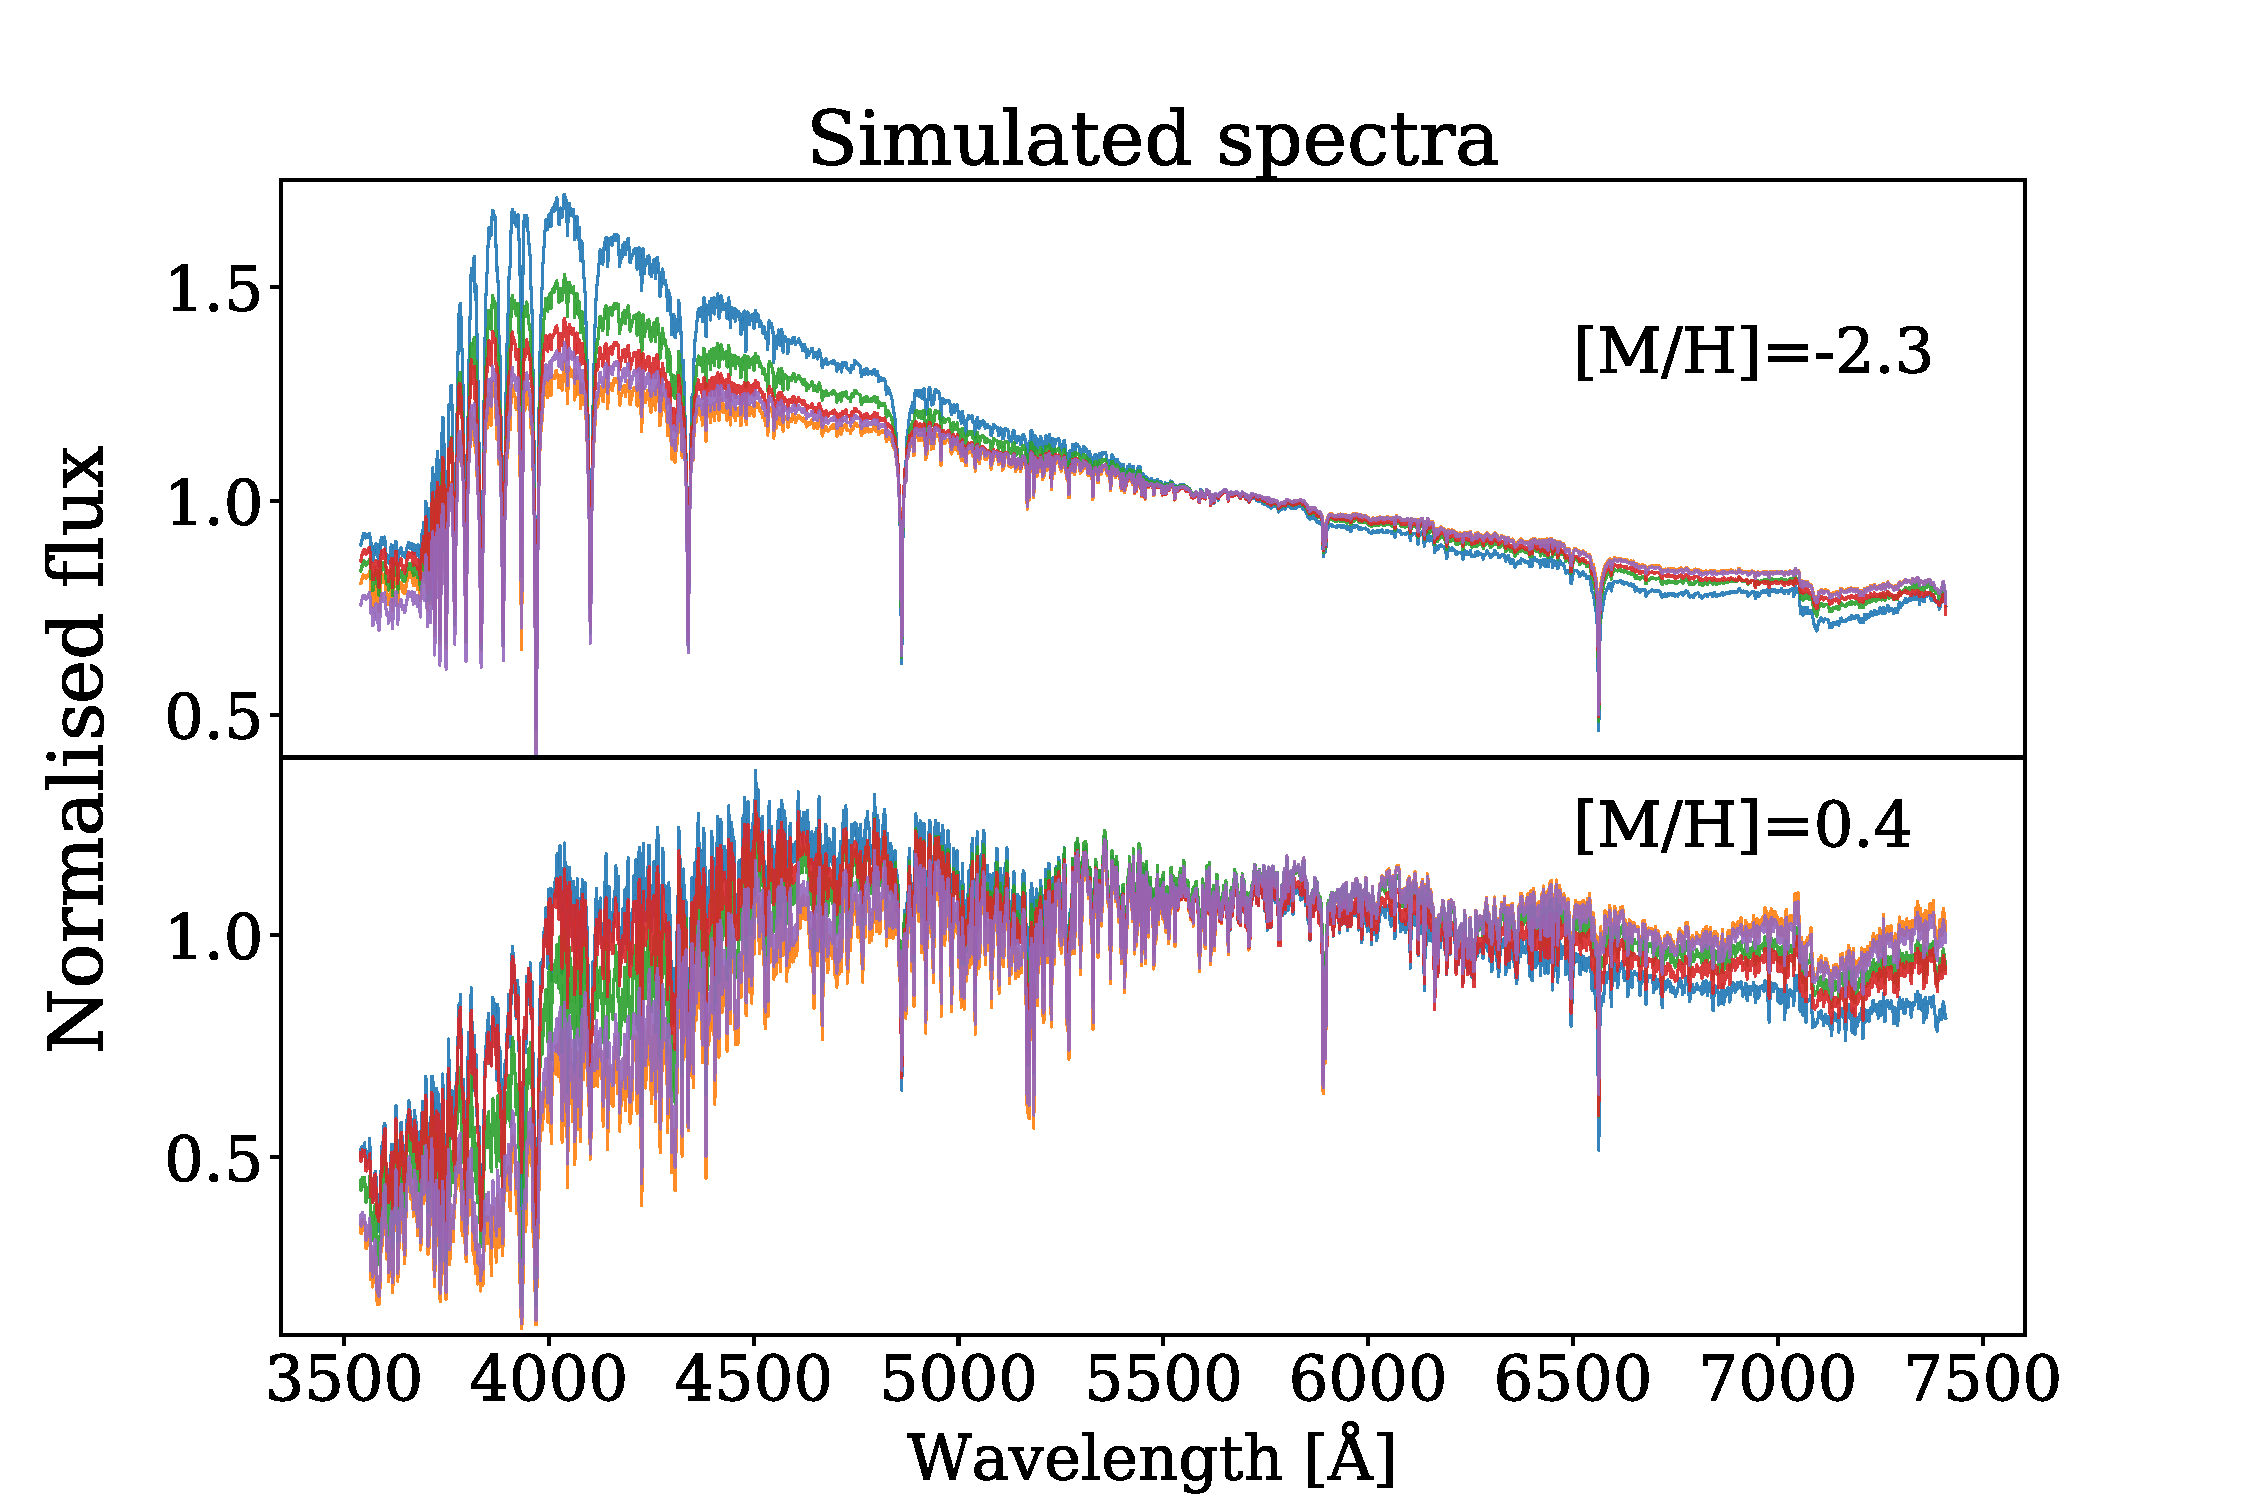
\includegraphics[width=0.49\textwidth]{images/input/sim_spectra.pdf}
    \caption{Samples of the simulated dataset, each of them with a different colour. In the left plot we show their mocked SFHs: in the upper panel the SFR normalised by the total stellar mass in Gyr$^{-1}$, and in the lower one the nine stellar mass percentiles, together with three dashed grey lines indicating when $25\%$, $50\%$ and $75\%$ of the total stellar mass has been formed. In the right plot, we show the  simulated normalised spectra corresponding to these SFHs using the same colours, for two different values of metallicity: in the upper panel we fix $\rm{[M/H]}=-2.3$, and in the lower one  $\rm{[M/H]}=0.4$, which are respectively the minimum and maximum bins of $\rm{[M/H]}$ in the simulation.}
    \label{input}
\end{figure*}


 Stellar mass curves, i.e. SFR as a function of time, are integrated to get nine stellar mass percentiles. We thus focus on the cosmic time,  i.e. the time since the Big Bang, at which $10$\%, $20$\%, ... $90$\%  of the total stellar mass of the galaxy has been formed. These quantities are more robust and smoother than their non-cumulative analogues, possibly relieving the effects imposed by the intrinsic priors of the simulation, so that the model inference is more stable. \\


\subsection{Backward Model}
\label{backward}
\subsubsection{Encoding the spectra}
\label{encoder}

High-quality absorption spectra typically cover, at least, a thousand $\AA$, described by a similar number of pixels. However, the widespread adoption of template libraries suggests that galaxy spectra in fact occupy a low-dimensional manifold. In particular, \cite{Portillo_2020} demonstrated that a high-fidelity reconstruction can be achieved by an autoencoder (AE) architecture  \citep{hinton}, a non-linear dimensionality reduction technique, with a latent space of just six dimensions. \cite{Teimoorinia_2022}  and  \cite{melchior2022} improved the method by introducing convolutional elements into the AE to aid the extraction of correlated features from the spectra. In short, AEs are feed-forward neural networks that learn efficient encodings of data in an unsupervised manner. They consist of two parts: an encoder, which takes data as input and compresses it to produce a low-dimensional latent representation, and a decoder, which takes the latent representations and decompresses them to reconstruct the original data. Due to their non-linear behaviour, AEs can capture non-linear features, such as line widths, with fewer parameters than principal component analysis (PCA) \citep{Yip_2004}, one of the most commonly used techniques. Moreover, unlike line-ratio diagnosis, AEs use the continuum information in the spectra, resulting in an interpretable latent space that shows clear separations between different classes of galaxies, even though they were never given these classifications in training.\\


We take advantage of this approach to obtain low-dimensional representations of the spectra, using the encoder part of the architecture implemented by \cite{melchior2022} (SPENDER). These representations are more suitable than the full spectrum to be introduced into a Bayesian inference model for a fully probabilistic treatment, and to perform meaningful summary statistics. The size of the latent representations is a tunable parameter and depends on what information in the spectrum is relevant to determine the SFHs and metallicity, as well as on the dimension of the spectrum and the performance required. During this work, it is set to $16$, as most of the details of the spectra that contain information relevant to the early star formation of galaxies are extremely subtle.\\

 Our network consists of a three-layer convolutional neural network (moving to wider kernels and including max-pooling), plus an attention module (dot-product), and a three-layer multi-layer perceptron (MLP), to obtain the latent vectors. Furthermore, an additional two-layer MLP is included to optimise the encoding for our final task: to obtain stellar mass percentiles and a value of $\rm{[M/H]}$, incorporating a log-cosh loss function. This computes the difference between the predicted and actual values, driving the evolution of the training. The encoder is trained with the training and validation sets ($80\%$ and $10\%$ of the total number of samples), and the training is stopped when the validation loss reaches a plateau, after 250 epochs approximately. Then, the model is applied to test data (the remaining $10\%$ of the total number of samples, never seen before by the network), producing not only the latent vectors we will use for the Bayesian inference, but also an initial prediction for the mass percentiles and metallicity that we can easily compare with the true ones. These predictions will not be used once we have trained the encoder: they only drive the training process, while the proper measurements of the galaxy properties will be done by the neural density estimator, as detailed below.\\





\subsubsection{Posterior estimation}
\label{normflows}


We use an Amortised Neural Posterior Estimation (ANPE) technique known as Normalising Flows, to estimate the posterior probability distribution for each of the stellar mass percentiles, and for the metallicity. In a few words, variables $(z)$ described by a simple base distribution $P(z)$, such as a multivariate Gaussian, are transformed through a parameterised invertible transformation $x=f(z)$, that has a tractable Jacobian. The target density $P_f(x)$ is then given by the change-of-variables formula as a product of the base density and the determinant of the transformation's Jacobian:

\begin{equation}
P_f(x)=P(z)\left|\operatorname{det} J_{f^{-1}(x)}\right|.
\end{equation}

Several such steps can be stacked, with the probability density `flowing' through the successive variable transformations. The parameters of the transformations during the training of the model are estimated by maximising the log likelihood of the transformed data under the Gaussian distribution $P(z)$, which is indeed tractable:

\begin{equation}
\log P_f(x)=\log P(f^{-1}(x))+\log \left|\operatorname{det} J_{f^{-1}(x)}\right|.
\end{equation}

Otherwise, it would not be possible to compute the loss since $P(x)$ is unknown. Following this pipeline, Normalising Flows have been generalised to model a conditional density such as  the posterior $P(\theta \mid x)$. Following the choice of \cite{Hahn_2022}, we develop a Masked Autoregressive Flow (MAF) \citep{papamakarios2018masked}, implemented with the module SBI \citep{tejerocantero2020sbi},  with five Masked Autoencoder for Distribution Estimation (MADE) blocks, each of them with two hidden layers of $128$ hidden units. In total, the model has a set of $50{,}560$ free parameters $\phi$. Our goal is to determine $\phi$ for the MAF model, so that given galaxy properties $\theta$ and observations $x$, $P_{\phi}\left(\theta \mid x \right)$ accurately estimates the posterior probability distribution $P\left(\theta \mid x \right)$.  In practice, we divide the training data into training and validation sets with a $90/10$ split. We use the Adam optimiser with a learning rate of $5\cdot 10^{-4}$. To prevent overfitting, we evaluate the likelihood of the data points under the base distribution, using the validation data at every training epoch, and stopping the training when that validation likelihood fails to increase after $20$ epochs.\\

 By using this workflow, we train our model with mock synthetic data, and then apply it to observations to obtain promptly posteriors for the SFHs and metallicity, thanks to its amortised\footnote{Not focused on any particular observation. Once we have a trained model, new data can be evaluated without repeating the training, the computationally expensive step.} nature.\\
 
 We are making two important assumptions. First, the simulator $F$ must be capable of generating mock data $x'$ that is practically indistinguishable from the observations $x$, which is the same requirement of any probabilistic modelling approach, but in contrast with likelihood-based evaluations, such as conventional MCMC, data generated need to include all relevant features one can find in spectra, such as noise or outliers. Second, the neural density estimator must be well trained, so  $P_f(\theta \mid x')$ is a good approximation of $P(\theta \mid x')$, and therefore of $P(\theta \mid x)$. As opposed to standard variational inference, we are not assuming any functional form for the posterior, and since neural networks are universal approximators, we could therefore estimate the posterior with an arbitrarily small error.\\


